\documentclass[12pt]{article}
\usepackage[margin=1in]{geometry}
\usepackage{setspace}
\usepackage{booktabs}
\usepackage{graphicx}
\usepackage{amsmath}
\usepackage{caption}

\onehalfspacing

\title{Assignment #1}
\author{}
\date{}

\begin{document}

\maketitle

\section{How did the AI coefficient change after applying PSM?}

The AI adoption coefficient decreased from 4.1427 in the naive OLS to 3.1164 after applying PSM matched, a reduction of approximately 1.03 percentage points, or about 25\% of the original estimate. Despite this reduction, the effect remains statistically significant (p = 0.015), suggesting that AI adoption has a genuine positive causal effect on firm revenue growth even after accounting for selection bias. The two regression results are summarized in Table 1.

\begin{table}[h!]
\centering
\caption{OLS vs PSM Matched Regression Results}
\begin{tabular}{lcccc}
\toprule
 & Coefficient & Std. Error & t-statistic & p-value \\
\midrule
\textbf{Naive OLS} & & & & \\
Constant  & 9.2800  & 0.551 & 16.840 & 0.000 \\
AI Status & 4.1427  & 0.997 & 4.155  & 0.000 \\
\midrule
\textbf{PSM Matched OLS} & & & & \\
Constant  & 10.2864 & 0.876 & 11.744 & 0.000 \\
AI Status & 3.1164  & 1.239 & 2.532  & 0.015 \\
\bottomrule
\end{tabular}
\end{table}

\section{What does this shift suggest about selection bias in AI impact stories?}

The downward shift in the coefficient after PSM suggests that positive selection bias was present in the naive estimate. Firms that adopted AI were already different from non-adopters and tended to be larger, spend more on R\&D, and have more customers. These characteristics independently contribute to higher revenue growth, which inflated the naive OLS estimate. By using PSM, the analysis makes a more fair comparison by matching AI-adopting firms with similar non-adopting firms. This helps isolate the actual effect of AI, leading to a more realistic estimate. In general, this highlights an important issue in the study of new technologies. Companies that adopt innovations early are often already better positioned to succeed. 

\section{Validity of the Common Support and Balancing Assumptions}

\subsection{Common Support}

The common support assumption appears to be satisfied. As shown in Figure 1, the propensity score distributions of treated and control firms overlap meaningfully in the 0.1–0.6 range, indicating that comparable control firms exist for most treated firms. The propensity scores range from 0.078 to 0.894, with a mean of 0.306. However, control firms are more heavily concentrated at lower propensity scores (0.1–0.3), suggesting that many non-adopting firms differ systematically from adopters in their observable characteristics. While this does not violate the common support assumption, it indicates that matches may be less precise at the extremes of the distribution. 

\begin{figure}[h!]
\centering
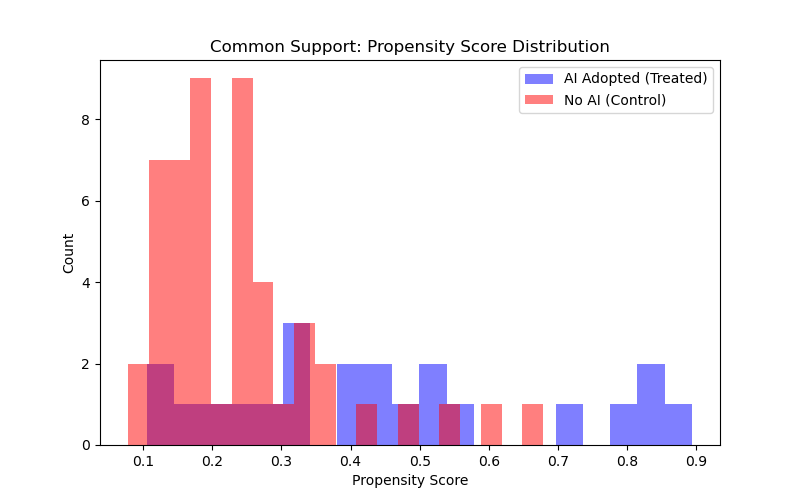
\includegraphics[width=0.8\textwidth]{common_support.png}
\caption{Common Support: Propensity Score Distribution by AI Adoption Status}
\end{figure}

\subsection{Balancing Property}

The balancing property is partially satisfied. Table 2 presents the Standardized Mean Differences (SMD) for each covariate before and after matching. Prior to matching, several covariates exhibited substantial imbalance. In particular, R\&D Spend had the largest SMD at 0.759, followed by Team Size (0.648) and Annual Revenue (0.588), indicating that AI-adopting firms were generally larger and more resource-intensive than non-adopters.

After applying nearest-neighbor propensity score matching, the SMD values moved significantly closer to zero across all covariates, demonstrating improved balance. R\&D Spend showed the most notable improvement, decreasing from 0.759 to -0.073. While some residual imbalance remains in variables such as Founded (-0.390) and Customer Accounts (-0.268), the overall reduction in SMD values suggests that the matching procedure was largely effective in creating more comparable groups.

 

\begin{table}[h!]
\centering
\caption{Standardized Mean Differences Before and After PSM Matching}
\begin{tabular}{lcc}
\toprule
Covariate & SMD Before Matching & SMD After Matching \\
\midrule
Team Size       & 0.6482  & 0.2935  \\
Founded         & 0.3547  & -0.3895 \\
Annual Revenue  & 0.5881  & -0.2122 \\
R\&D Spend      & 0.7590  & -0.0730 \\
Digital Sales   & 0.3568  & -0.2031 \\
Customer Accts  & 0.3947  & -0.2683 \\
\bottomrule
\end{tabular}
\end{table}

\end{document}
